\documentclass[12pt,a4paper]{article}
\usepackage{inverba}

\newcommand{\userName}{Cullyn Newman} 
\newcommand{\class}{CH 334} 
\newcommand{\institution}{Portland State University} 
\newcommand{\theTitle}{\color{B-Cold} Organic Chemisty}

\begin{document}
%%%%%%%%%%%%%%%%%%%%%%%%%%%%%%%%%%%%%%%%%%%%%%%%%%%%%%%%%%%%%%%%%%%%%
\tableofcontents
\cleardoublepage
\fancyhead{}
\fancyhead[R]{\hyperlink{home}{\nouppercase\leftmark}}
%%%%%%%%%%%%%%%%%%%%%%%%%%%%%%%%%%%%%%%%%%%%%%%%%%%%%%%%%%%%%%%%%%%%%

\clearpage
%\begingroup
%%%%%%%%%%%%%%%%%%%%%%%%%%%%% Chapter 1 %%%%%%%%%%%%%%%%%%%%%%%%%%%%%
%\begingroup
\clearpage
\section{General Chemistry Review}\phantomsection
\subsection{Electrons, Bonds, and Lewis Structures}
\begin{itemize}
    \item \textbf{Covalent bond}: two atoms sharing a pair of electrons.
    \item \textbf{Octet rule}: \textit{main group elements} that tend to bond in a way that each atom has {\color{o-Sun}eight} electrons in it's valence shell.
        \begin{itemize}
            \item Atoms that do not have eight will share electrons with other elements in order to maintain a stable state.
        \end{itemize}
    \item \textbf{Main group elements}: sometimes called representative elements, are groups 1, 2 and 13--18 in periodic table.
        \begin{itemize}
            \item Some elements in group 3 and 12 share properties between transition metals and the main group.
        \end{itemize}
    \item The lowest energy (most stable) state of two atoms is determined both by bond length and bond strength.
    \item Valence electrons are determined by the group, 1A--8A, of the periodic table.
    \item \textbf{Lone pair}: unshared, or nonbonding, electrons.
    \item \textbf{Lewis structures}: 2D model that represnets covalent bonds as straight lines and lonpairs as dots.
    \item Examples: \ch{COF2}, \ch{H2O}, \ch{NO3-}, \ch{N2O}:
        \begin{align*}
            \chemfig{C(=[2,.8]O)(-[5]F)(-[7]F)}
            \hspace{1cm}
            \chemfig{[:40]H-\lewis{13,O}-[::-80]H} 
            \hspace{1cm}
            \left[\chemfig{N(=[2,.8]O)(-[5]O)(-[7]O)}\right]^{-1} 
            \hspace{1cm}
            \chemfig{N(~[4]N)(-[0]O)}
        \end{align*}
    \item \textbf{Resonance structures}: a set of two or more Lewis structures that collectively describe the electronic bonding of a single polyatomic species, including fractional bonds.
\end{itemize}

\subsection{Identifying Formal Charges}
\begin{itemize}
    \item \textbf{Formal charge}: any atom that does not exhibit the appropriate number of valance electrons.
    \item Determing formal charge:
        \begin{itemize}
            \item Formula: {\color{o-Sun}\(FC = V - N - \dfrac{B}{2}\)}
            \item V = valance electrons of element
            \item N = lone pair electrons
            \item B = bonded electrons
        \end{itemize}
    \item {\color{pos}Less} than expected number of valence electrons results in a {\color{pos} positive} charge.
    \item {\color{neg}More} than expected number of valence electrons results in a {\color{neg}negative} charge.
    \item The lower the {\color{o-Sun}magnitude} of formal charge, the {\color{o-Sun}greater the stability} of the whole molecule.
    \item Atoms that are {\color{neg}more electronegative} hold {\color{neg}negative} formal charges better, which results in {\color{o-Sun}greater stability} vs when the negative charge is spread on less electronegative elements in a polyatomic species.
        \begin{itemize}
            \item The dominant resonance structure will be that of the greatest stability. 
        \end{itemize}
\end{itemize}

\subsection{Induction and Polar Covalent Bonds}
\begin{itemize}
    \item Bonds can classified into three categories: covalent, polar covalent, and ionic.
    \item The categories emerge from the electronegativity values of the atoms sharing a bond.
    \item \textbf{Electronegativity}: a measure of the ability of an atom to attract electrons.
        \begin{itemize}
            \item Electronegativity generally {\color{o-Sun}increases left to right}, and from the {\color{o-Sun}bottom to top} of the periodic table.
            \item \textbf{F, O, N, Cl} (Br, I). Most electronegative elements, from left to right, that are often encountered.
        \end{itemize}
    \item \textbf{Covalent bond}: when the difference in electronegativity is {\color{o-Sun}less than 0.5}.
    \item \textbf{Polar covalent bond}: when the difference in electronegativity is {\color{o-Sun}between 0.5 and 1.9}, then the electrons are not equally shared and become polar.
    \item \textbf{Induction}: the withdrawl of electrons towards to more electronegative atom. {\color{pos}\ch{$\delta$^+}} represnets partial positive charged gained when electrons are pulled away, while {\color{neg}\ch{$\delta$^-}} represnets the partial negative charge pulled closer.
    \item \textbf{Ionic bond}: when the difference in electronegativity is {\color{o-Sun}greater than 1.9}.
        \begin{itemize}
            \item Electrons are not shared in this case, and attraction is insetsad just the result of oppositely charged ions.
        \end{itemize}
\end{itemize}

\subsection{Atomic Orbitals}
\begin{itemize}
    \item \textbf{Atomic orbital (AO)}: standing quantum wave (excitation in electron field) around an atom.
    \begin{itemize}
            \item More energy leads to higher orbtails levels.
                \begin{itemize}
                    \item Gives principle quantum number, \(n\), as is associated with distance from nucleus.
                \end{itemize}
            \item Orbital levels: s(1 pair), p(3 pairs), d(5 pairs), f(7 pairs). 
                \begin{itemize}
                    \item Angular momentum quantum number that describes three-dimensional region of space that the electron density occupies.
                \end{itemize}
            \item Magnetic quantum number descrices orientation in space of electron density.
                \begin{itemize}
                    \item \(m_l=0\); s orbital
                    \item \(m_l=-1, 0, 1\); p\(_{x}\), p\(_{y}\), p\(_{z}\) orbitals.
                \end{itemize}
            \item Locations where $\psi$ (quantum wave function) is zero are called \textbf{nodes}.
                \begin{itemize}
                    \item The {\color{o-Sun}more nodes} that an orbital has, the {\color{o-Sun}greater} it's energy.
                \end{itemize}
            \item \textit{Spin}: allows an orbital to contain only two electrons, \(\pm \frac{1}{2}\)
        \end{itemize}
    \item \textbf{Degenerate orbitals}: orbitals with the same energy level.
    \item Order in which orbitals are filled is determined by three principles:
        \begin{itemize}
            \item \textbf{Aufbau principle}: lowest energy orbital is filled first.
            \item \textbf{Pauli exclusion principle}: each orbital can accommodate a maximum of two electrons that have opposite spin.
            \item \textbf{Hund's rule}: electrons are placed in each degenerate orbital before being paired up.
        \end{itemize}
    \item Describing the nature of atomic orbital is done with two commoly used theories: \textit{Valence Bond Theory} and \textit{Molecular Orbital Theory}.
    \item The commonly used theories give a deeper understanding of covalent bonds, which is essentially just the {\color{o-Sun}overlap of atomic orbitals}.
    \item \textbf{Constructive/destructive interference}: the result of two waves that approach each other, or overlap.
        \begin{itemize}
            \item Constructive interference produces a wave with the vector sum of both waves.
            \item Destructive interference cancel each other out and produes a node.
        \end{itemize}
\end{itemize}


\subsection{Valence Bond Theory}
\begin{itemize}
    \item \textbf{Valence bond theory}: the sharing of electron density between two atoms is a result of the constructive interference of their atomic orbitals.
    \item \textit{Bond axis}: the line that can be drawn between two hydrogen atoms.
    \item \textbf{Sigma bond (\(\bm{\sigma}\))}: a particular type of covalent bond that has circular symmetry with respect to the bond axis.
        \begin{itemize}
            \item All single bonds are $\sigma$ bonds.
            \item The strongest type of covalent bond.
        \end{itemize}
    \item \textbf{Pi bond ($\bm{\pi}$)}: covalent bonds where two lobes of an orbital overlap with two lobes of another atom. 
        \begin{itemize}
            \item Each atomic orbital has zero electron density at a shared nodal plane, passing through the two bonded nuclei.
            \item $\pi$ bonds form double ($\sigma + \pi$) and triple bonds ($\pi + \sigma + \pi$).
            \item Individual $\pi$ bonds are weaker than $\sigma$ bonds.
        \end{itemize}
\end{itemize}

\subsection{Molecular Orbital Theory}
\begin{itemize}
    \item \textbf{Molecular orbital theory (MO)}: uses linear combinations of atomic orbitals to model and explore the consequences of orbital overlap.
        \begin{itemize}
            \item The newly described orbitals are called {\color{o-Sun}molecular orbitals} accroding to MO theory.
        \end{itemize}
    \item Atomic orbitals refer to an individual atom, while molecular orbitals is associated with an entire molecular.
    \item In other words, MO theory states that atomic orbitals cease to exist when they overlap. Instead they are replaced with multiple molecular orbitals which span the entire molecule.
    \item Molecular orbitals are more stable (lower energy) since electrons are attracted by both nuclei.
    \item When there are {\color{o-Sun}nodes} between the nuclei, then the resulting $\sigma^*$ orbitals become {\color{o-Sun}antibonding}, as they {\color{o-Sun}destabilize} (increase the energy) of a molecular orbital.
    \item Best used to produce a quantitative picture of bonding.
        \begin{itemize}
            \item Describes strength, order, and polarity of bonds.
            \item Allows for the presence of paired or unpaired electrons.
            \item Has spectroscopic preperties.
        \end{itemize}
\end{itemize}

\subsection{Hybridized Atomic Orbitals}
\begin{itemize}
    \item \textbf{sp\(\bm{^3}\)-hybridized orbitals}: produced by averaging one \textit{s} orbital and {\color{o-Sun}three} \textit{p} orbitals.
        \begin{itemize}
            \item Hybridized orbitals explains to geomtry of methane, which results form the {\color{o-Sun}now four degenerate} orbitals pushing apart to achieve tetrahedral geometry.
            \item Hybridized orbitals become {\color{o-Sun}unsymmetrical}, producing a larger front lobe that is more efficient than standard \textit{p} orbitals in the ability to form bonds.
            \item All bonds in are {\color{o-Sun}$\sigma$ bonds}, and thus can be individually represented by the overlap of atomic orbitals.
        \end{itemize}
    \item \textbf{sp\(\bm{^2}\)-hybridized orbitals}: produced by averaging the \textit{s} orbital with only {\color{o-Sun}two} of \textit{p} orbitals.
        \begin{itemize}
            \item The remaining \textit{p} orbital is unaffected, and free multiple p orbitals results in a $\pi$ bond.
            \item This is done to expain geometry of compounds bearing a double bond.
            \item A double bond if formed from one $\sigma$ bond and one $\pi$ bond.
            \item Associated with \textit{trigonal planar geometry}.
        \end{itemize}
    \item \textbf{sp-hybridized orbitals}: produced by averaging of one \textit{s} orbital and {\color{o-Sun}one} \textit{p} orbital.
        \begin{itemize}
            \item Leaves two \textit{p} orbitals and resulting in two $\pi$ bonds.
            \item A triple bond is formed with the addition of one $\sigma$ bond due to the overlap of the sp orbitals.
            \item Geometry of a triple bond has \textit{linear geometry}.
        \end{itemize}
    \item Finding the hybridization of any atom can be done simply: 
        \begin{itemize}
            \item[1.] Look at the central item.
            \item[2.] Determin groups (number of bonds, $\pi$ bonds count as 1, and lone pairs attached) of atom.
                    \begin{itemize}
                        \item groups aka regions of electron density.
                    \end{itemize}
            \item[3.] For groups 1-4: sp\(^{x}\); x = groups - 1  
            \item[4.] For groups 5-6: sp\(^{3}\)d\(^{x}\); x = groups - 4 
        \end{itemize}
    \item Bond Strength and Bond Length:
        \begin{itemize}
            \item Bond length {\color{neg}decreases} with more bonds.
            \item Bond strength {\color{pos}increases} with more bonds.
            \item The more {\color{o-Sun}\textit{s} character}, the {\color{pos}shorter} and {\color{pos}stronger} the bond, and the {\color{pos}larger} the bond angle.
                \begin{itemize}
                    \item \textit{s-character}: contribution of the $\sigma$ bond in a hybridization.
                        \begin{itemize}
                            \item e.g. sp = 50\%, sp\(^{2}\) = 33\%, sp\(^{3}\) = 25\%
                        \end{itemize}
                    \item sp-sp bond is the strongest, sp\(^{3}\)-sp\(^{3}\) is the weakest.
                \end{itemize}
        \end{itemize}
\end{itemize}

\subsection{Molecular Geometry}
\begin{itemize}
    \item \textbf{Valence shell electron pair repulsion (VSEPR) theory}: enables the {\color{o-Sun}prediction of molecular geometry} due to the pressumption that all electron pairs repel each other; resulting in a three-dimensional space that {\color{o-Sun}maximizes distance} from each other.
    \item \textbf{Steric number}: the total number of electron pairs in a molecule. Can be bonds or lone pairs.
    \item \textbf{Tetrahedral geometry}: result of four $\sigma$ bonds and zero lone pairs. 
        \begin{itemize}
            \item produces a tetrahendron with bond angles of \ang{109.5}.
        \end{itemize}
    \item \textbf{Trigonal pyramidal geometry}: three $\sigma$ bonds and one lone pair.
        \begin{itemize}
            \item The lone pair occupy more space than bonded electron pairs, so the remaining angles are slightly less than a tetrahedral, at \ang{107}.
            \item The lone pair sits atop the base forming a pyramid like structure.
        \end{itemize}
    \item \textbf{Bent geometry}: two $\sigma$ bonds and two lone pairs.
        \begin{itemize}
            \item VSEPR predicts the lone pairs to be in two corners of the tetrahedral, producing bond angles of \ang{105}.
            \item VSEPR predicts geometry \ch{H2O} correctly, but for wrong reasons.
                \begin{itemize}
                    \item The lone pairs in \ch{H2O} have different energy levels, suggesting one pair occupies a \textit{p} orbital with the other in a lower-energy hybridized orbital.
                \end{itemize}
        \end{itemize}
    \item VSEPR theory is best used for a first approximation and is mostly accurate for most small molecules.
    \item \textbf{Trigonal planar geometry}: three electron pairs forming three bond angles of \ang{120} and lie on the same plan. 
    \item \textbf{Linear geometry}: two electron pairs that oppose each other at \ang{180}, forming a linear structure.
    \item General method of determining structure:
    \begin{itemize}
        \item[1.] Count steric number---the total number of electron pairs in a molecule. Can be bonds or lone pairs.
        \item[2.] Determine predicted geomterical structure predicted (EDG) by VSEPR using steric number.
            \begin{itemize}
                \item Octahedral:6, Bipyramid:5, Tetrahedral:4, Trigonal:3, Linear:2
            \end{itemize}
        \item[3.] Determin impact (the MG) of lone pairs; more lone pairs results in less space between bonded pairs. Shape depends on EDG.
    \end{itemize} 
\end{itemize}

\subsection{Dipole Moments and Molecular Polarity}
\begin{itemize}
    \item \textbf{Dipole moment} ($\bm{\mu}$): defined as the amount of partial charge, $\delta$, on on either end of the dipole multiplied by the distance separtion, d:
        \begin{itemize}
            \item {\color{o-Sun}\(\mu=\delta d\)}
            \item $\mu$ generally has an order of magnitude of {\color{o-Sun}\SI{e-18}{esu.cm}} due to general partial charge (esu) and distance (cm) values.
            \item 1 {\color{o-Sun}debye (D)} = \SI{e-18}{esu.cm} 
        \end{itemize}
    \item \textbf{Molecular dipole moment}: the vector sum of the individual dipole moments.
        \begin{itemize}
            \item Lone pairs have significant effect on the molecular dipole moment.
            \item Also called the net dipole moment.
        \end{itemize}
\end{itemize}

\subsection{Intermolecular Forces and Physical Properties}
\begin{itemize}
    \item \textbf{Intermolecular forces}: the attractive forces between individual molecules that determed the physical properties of a compound.
    \item \textit{Electrostatic}: forces that occur as a result of the attraction between opposite charges. 
    \item Electrostatic interactions for neutral molecules (no formal charge) are often classified as into the following categories:
        \begin{itemize} 
            \item \textbf{Dipole-dipole interaction}: Compounds with  {\color{o-Sun}net dipole} moments. 
                \begin{itemize}
                    \item In {\color{o-Sun}solid} space these intereactions either {\color{o-Sun}repel or attract} each other.
                    \item In {\color{o-Sun}liquid} space these interactions tend to {\color{o-Sun}attract more often}, raising melting/boiling point.
                    \item \textbf{Ion-dipole}: electrostatic interaction between an ion and a molecule with a dipole.
                \end{itemize}
            \item \textbf{Hydrogen bonding}: molecules with a hydrogen attached to an F, O, or N.
                \begin{itemize}
                    \item Not actually a bond, just an interaction.
                    \item When hydrogen bonds to a electronegative atom, then the hydrogen will have a {\color{pos}$\delta^+$}.
                    \item Hydrogen bonding is strong due to size of hydrogen atom, resulting in very close partial charge interactions.
                    \item The {\color{o-Sun}more} hydrogen bonds, the {\color{o-Sun}higher} the boiling point tends to be.
                    \item Stronger than dipole-dipole interactions.
                \end{itemize}
            \item \textbf{Fleeting dipole-dipole interactions}:
                \begin{itemize}
                    \item Electrons are considered to be in constant motion, which restult in the center of negative charge to vary.
                    \item \textbf{London Dispersion Forces (LDFs)}: On average, the dipole moment is zero, though it can experience transient dipole moments, initiating fleeting attraction/repulsion.
                        \begin{itemize}
                            \item All atoms and molecules have LDFs.
                            \item Weakest, but the dominant force in non-polar molecules.
                            \item Dispersion forces directly related to molar mass.
                        \end{itemize}
                    \item Heavier hydrocarbons generally experience a stronger force due to increased surface area, and thus greater chance for non-zero dipole moments, which results in higher boling points.
                    \item Branched hydrocarbons generally have decreased surface area, decreasing boiling point relative to others of similar weight.
                \end{itemize}
        \end{itemize}
    \item When comparing boling points of compounds, look for following factors:
        \begin{itemize}
            \item Any dipole-dipole interactions? (increases boiling point)
            \item Formation of hydrogen bonds? (increase boling point)
            \item Number of electrons. (more electrons, higher boiling point)
            \item Number of carbon atoms. (more surface area, higher boiling point)
            \item Degree of branching of compound. (more branching, more surface area)
        \end{itemize}
\end{itemize}

\subsection{Structural Theory of Matter}
\begin{itemize}
    \item \textbf{Constitutional isomers}: aka structural isomers; same {\color{o-Sun}chemical formula}, but different in the way the {\color{o-Sun}atoms are connect}, i.e. their constitution is different.
        \begin{itemize}
            \item Consistenet with the octet rule.
            \item Each element forms a predictable number of bonds, from one to four.
            \item The number of {\color{pos}possbile constitutional isomers increases} as the number of {\color{pos}carbon atoms increases}
        \end{itemize}
    \item \textbf{Stereoisomers}: isomers that differ in {\color{o-Sun}spatial arrangement} of atoms, rather than connectivity.
        \begin{itemize}
            \item \textbf{Geometric isomerism}: aka cis--trans; {\color{o-Sun}locked into spatial positions} due to double bonds or a ring structure.
                \begin{itemize}
                    \item Cis indicates functional groups that are on the same side of the carbon chain.
                    \item Trans indicates functional groups on opposite sides of the carbon chain.
                \end{itemize}
            \item \textbf{Enantiomers}: aka optical isomers; mirror images of each other that are non-superposable.
                \begin{itemize}
                    \item Human hands are a macroscopic analogy.
                \end{itemize}
        \end{itemize}
    \item \textit{More detail will be covered in later sections.}
\end{itemize}
%\endgroup
%%%%%%%%%%%%%%%%%%%%%%%%%%%%% Chapter 1 %%%%%%%%%%%%%%%%%%%%%%%%%%%%%

%%%%%%%%%%%%%%%%%%%%%%%%%%%%% Chapter 2 %%%%%%%%%%%%%%%%%%%%%%%%%%%%%
%\begingroup
\clearpage
\section{Molecular Representations}\phantomsection
\subsection{Types of Molecular Representations}
\begin{itemize}
    \item \textbf{Partially condensed structures}: the \ch{C-H} bonds are not always drawn, saving space.
        \begin{itemize}
            \item \small\chemfig{C(-[4]CH_3)(-[2]OH)(-[0]CH_3)(-[6]H)}
        \end{itemize}
    \item \textbf{Condensed structures}: single bonds are not drawn and groups of atoms are clustered when possbile.
        \begin{itemize}
            \item \ch{CH3CH3CHOH -> (CH3)2CHOH}
        \end{itemize}
    \item \textbf{Molecular formula}: simply shows number of each type of atom with no structural information.
        \begin{itemize}
            \item \ch{C3H8O}
        \end{itemize}
    \item Example of converting a condensed structure into a partially condensed structure:
        \begin{itemize}
            \item ({\color{o-Sun}CH\(_{3}\)})\(_{3}\){\color{Liblue}CC}H\(_{2}\){\color{Liblue}C}H({\color{o-Sun}CH\(_{3}\)}){\color{Liblue}C}H({\color{o-Sun}CH\(_{3}\)}){\color{Liblue}C}H({\color{o-Sun}CH\(_{3}\)})\(_{2}\)
            \item \chemfig{{\color{Liblue}C}(-[4]{\color{o-Sun}CH_3})(-[6]{\color{o-Sun}CH_3})(-[2]{\color{o-Sun}CH_3})
            (-[0]{\color{Liblue}C}(-[6]H)(-[2]H)
            (-[0]{\color{Liblue}C}(-[6]{\color{o-Sun}CH_3})(-[2]H)
            (-[0]{\color{Liblue}C}(-[6]{\color{o-Sun}CH_3})(-[2]H)
            (-[0]{\color{Liblue}C}(-[6]{\color{o-Sun}CH_3})(-[2]H)(-[0]{\color{o-Sun}CH_3})
            ))))}
            \item This shows just one isomer, more partially condensed structures are possible.
        \end{itemize}

    \subsubsection{Bond-Line Structures}
    \begin{itemize}
        \item \textbf{Bond-line structures}; aka skeletal structures; simplify drawing process of chemical structures and are easier to read.
        \item Each corner or endpoint represents a carbon atom.
            \begin{itemize}
                     \item {\tiny\chemfig{-[:30]-[:-30]-[:30]-[:-30]-[:30]}
                     \hspace{15pt}
                     \chemfig{-[:30](-[:90])-[:-30]-[:30]-[:-30]}
                     \hspace{15pt}
                     \chemfig{-[:30](-[:90])-[:-30](-[:-90])-[:30]}}
                     \item All examples have 6 carbon atoms
            \end{itemize}
        \item Double bonds are shown with two lines, triple with three.
            \begin{itemize}
                \item {\tiny\chemfig{-[:30]=_[:-30]-[:30]}
                \hspace{15pt}
                \chemfig{-[:30]~[:30]-[:30]}}
                \item Triple bonds are drawn linearly due to sp-hybridization
            \end{itemize}
        \item Hydrogens are not shown; it is assumed that each carbon posses enough to satisfy octet rule.
    \end{itemize}
    \subsubsection{Notes on Drawing Bond-Line Structrues}
    \begin{itemize}
        \item Carbon atoms in a straight chain should be drawn in zigzag format in order to accurately show each carbon.
        \item Double bonds should be drawn as far apart as possible:
            \begin{itemize}
                \item {\tiny\chemfig{-[:30](=[:90]O)-[:-30]}} = good
                \hspace{20pt} {\tiny\chemfig{-[:30](=[:-90]O)-[:-30]}} = bad
            \end{itemize}
        \item Direction of a single bond is irrelevant:
            \begin{itemize}
                \item {\tiny\chemfig{-[:-30]-[:30](-[:90])-[:-30]-[:30]}}
                \hspace{12pt} is the same as \hspace{12pt} {\tiny\chemfig{-[:-90]-[:30](-[:90])-[:-30]-[:90]}}
            \end{itemize}
        \item All {\color{o-Sun}heteroatoms} (atoms other than carbon and hydrogen) must be drawn.
            \begin{itemize}
                \item Hydrogens next to heteroatoms must be shown.
            \end{itemize}
        \item Carbons cannot have more than four bonds.
    \end{itemize}
\end{itemize}

\subsection{Hydrogen Deficiency Index: Degrees of Unsaturation}
{\color{G-Moon}\textit{Excerpt from Chapter 14: Infrared Spectroscopy and Mass Spectrometry}}
\begin{itemize}
    \item \textbf{Saturated compounds}: the maximum number of hydrogen atoms possbile, relative to number of carbon present.
        \begin{itemize}
            \item Determining saturation using molecular formula: {\color{o-Sun}C\(_{n}\)H\(_{2n+2}\)}~~\(n=\) carbon atoms
        \end{itemize}
            \begin{itemize}
                \item \textbf{Halogens}: takes the place of a hydrogen atom; {\color{o-Sun}add one H} for each halogen.
                \item \textbf{Oxygen}: no affect on saturation; {\color{o-Sun}ignore}.
                \item \textbf{Nitrogen}: needs an extra hydrogen; {\color{o-Sun}subtract one H} for each nitrogen. 
            \end{itemize}
    \item \textbf{Unsaturated compounds}: a compound that contains at least one $\pi$ bond, resulting fewer than the maximum number of hydrogen atoms.
        \begin{itemize}
            \item Compounds with rings also result in an unsaturated compound.
            \item \textbf{Degree of unsaturation}: a number that represnets {\color{o-Sun}half} the {\color{o-Sun}"missing"} number of hydrogen atoms when compared to a saturated compound.
        \end{itemize}
    \item \textbf{Hydrogen deficiency index (HDI)}: the measure of degrees of unsaturation. 
        \begin{itemize}
            \item e.g. two degrees of unsaturation results in a HDI of 2.
            \item Degrees of freedom help represent possbile structures, indicating possible double bounds, triple bounds, rings, or various combinations of each.
            \item Only helpful when molecular formula is known for certainty.
            \item Formula: {\color{o-Sun}HDI = \(\frac{1}{2}(2C + 2 + N - H - X)\)}
            \begin{itemize}
                \item \(X\): halogen atoms.
        \end{itemize}
    \end{itemize}
\end{itemize}

\subsection{Identifying Functional Groups}
\begin{center}
    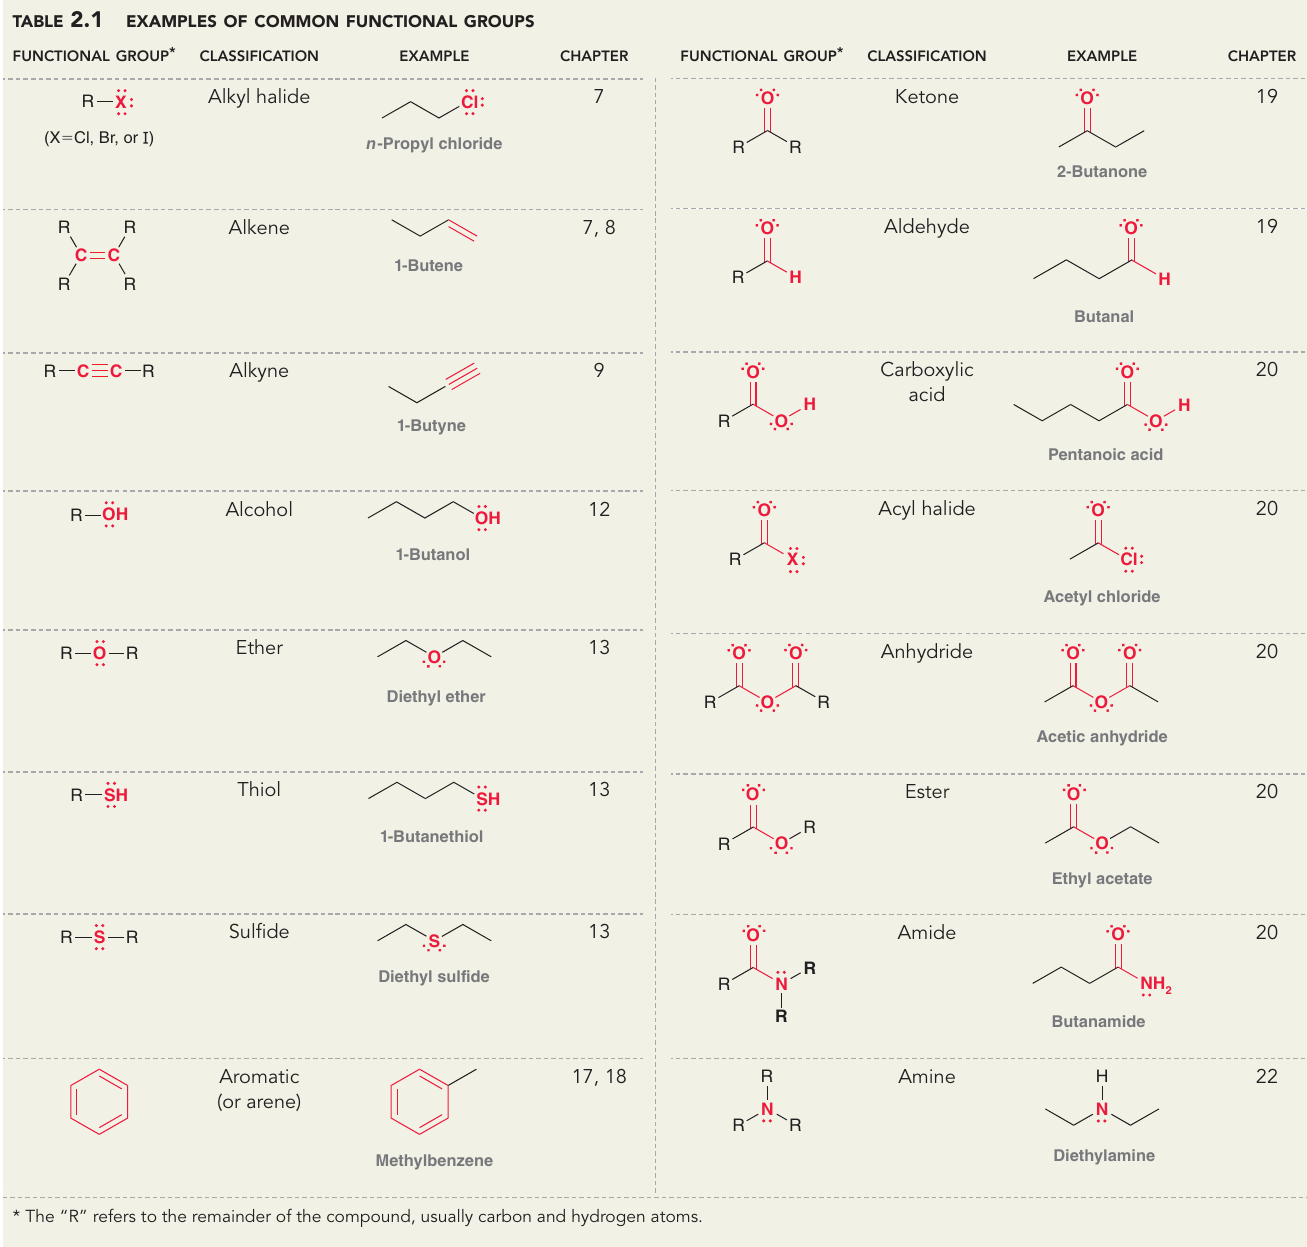
\includegraphics[scale=0.41]{images/fig2-1.png}
\end{center}
\begin{itemize}
    \item \textbf{Functional group (R)}: specific substituents or moieties within molecules that may be responsible for the characteristic chemical reactions.
        \begin{itemize}
            \item \textbf{Substituents}: an atom or group of atoms which replaces one or more hydrogen atoms on the parent hydrocarbon chain.
            \item \textbf{Moiety}: a part of a molecule which is typically found within other molecules and often given a specific name.
        \end{itemize}
    \subsubsection{Characterizing Carbon Centers and Functional Groups}
    \begin{itemize}
        \item \textbf{Characterizing Carbon Centers}
            \begin{itemize}
                \item Primary \ang{1}: a carbon with only one carbon-carbon bond.
                    \begin{itemize}
                        \item \ch{H3C-CH3}\hspace{12pt}\chemfig{-[:30]\ang{1}}
                    \end{itemize}
                \item Secondary \ang{2}: a carbon with two carbon-carbon bonds.
                    \begin{itemize}
                        \item \ch{H3C-CH2-CH3}\hspace{12pt}\chemfig{-[:30]\ang{2}-[:-30]}
                    \end{itemize}
                \item Tertiary  \ang{3}: a carbon with 3 carbon-carbon bonds.
                    \begin{itemize}
                        \item \ch{(CH)3-CH}\hspace{12pt}\chemfig{-[:30]\ang{3}(-[:90])-[:-30]}
                    \end{itemize}
                \item Quaternary \ang{4}: a carbon with four carbon-carbon bonds.
                    \begin{itemize}
                        \item \ch{(CH)4-C}\hspace{12pt}\chemfig{-[:30]\ang{4}(-[:135])(-[:45])-[:-30]}
                    \end{itemize}
            \end{itemize}
        \item \textbf{Characterizing Functional Groups}
            \begin{itemize}
                \item Certain functional groups can be characters as \ang{1}, \ang{2}, or \ang{3}, based on how many carbon bonds are attached to the carbon with the functional group.
            \end{itemize}
    \end{itemize}
\end{itemize}

\subsection{Identifying Lone Pairs}
\begin{itemize}
    \item Formal charges must always be drawn on bond line structures, otherwise the resulting bond line strcutres would be inferred incorrectly.
    \item Lone pairs do not have to be drawn and usually are omitted.
    \item The formal charge allows you to determin lone pairs.
        \begin{itemize}
            \item Formula: \(FC = V - N - \dfrac{B}{2}\)
            \item V = valance electrons of element
            \item N = lone pair electrons
            \item B = bonded electrons
            \item Solve for lone pairs: {\color{o-Sun}\(N = V - FC - \dfrac{B}{2}\)}
        \end{itemize}
    \item Frequent usage will allow for intuition for lone pairs.
    \newpage
    \subsubsection{Common Patterns Between Formal Charge and Lone Pairs}
    \begin{itemize}
        \item \textbf{Associated Patterns for Oxygen}
            \begin{itemize}
                \item A {\color{neg}negative ($\circleddash$)} charge corresponds with {\color{o-Sun}1 bond} and {\color{o-Sun}3 lone pairs}.
                \item The {\color{G-Moon}absence} of charge corresponds with {\color{o-Sun}2 bonds} and {\color{o-Sun}2 lone pairs}.
                \item A {\color{pos}positive ($\oplus$)} charge corresponds with {\color{o-Sun}3 bonds} and {\color{o-Sun}1 lone pair}.
            \end{itemize}
        \item \textbf{Associated Patterns for Nitrogen}
            \begin{itemize}
                \item A {\color{neg}negative} charge corresponds with {\color{o-Sun}2 bonds} and {\color{o-Sun}2 lone pairs}.
                \item The {\color{G-Moon}absence} of charge corresponds with {\color{o-Sun}3 bonds} and {\color{o-Sun}1 lone pair}.
                \item A {\color{pos}positive} charge corresponds with {\color{o-Sun}4 bonds} and {\color{o-Sun}0 lone pairs}.
            \end{itemize}
    \end{itemize}
\end{itemize}

\subsection{Resonance}
\begin{itemize}
    \item \textbf{Resonance}: description of bonding in molecules or ions by the combination of multiple contributing strcutres.
            \begin{itemize}
            \item \textbf{Resonance structures}: each contributing structure of the resonance hybrid.
                \begin{itemize}
                    \item Formal charges are important to include when drawing resonance structures as it clarifies where locations of lone pairs and movement of electrons.
                    \item Total charge must remain the same between structures.
                \end{itemize}
        \end{itemize}
    \item Resonance does not describe any real process, rather it's a method to overcome inadequacy of bond-line drawings.
    \item Different from isomerism, which differs in arrangements of atomic nuclei in space, rather than how the electrons are assigned to the depictions.
    \subsubsection{Resonance: Curved Arrows}
    \begin{itemize}
        \item \textbf{Curved arrows}: a tool used to help draw resonance strcutres by {\color{o-Sun}representing electrons as if} they were moving.
            \begin{itemize}
                \item Somwhat different from curved arrow notation in reactions, which actually represent the flow of electron density.
                \item Can help shows how to change the formal charge:
                    \begin{itemize}
                        \item Formal charges at the {\color{o-Sun}tail} become more {\color{pos}positive}, since it's losing an electron.
                        \item Formal charges at the {\color{o-Sun}head} more {\color{neg}negative}, since it's gaining an electron.
                    \end{itemize}
            \end{itemize}
        \item {\color{o-Sun}Avoid breaking a single bond}.
            \begin{itemize}
                \item Structures must have atoms connected in same order, though there are minor exceptions that \textit{will be discussed later}.
                \item This rule affects the placement of the {\color{o-Sun}tail} of the arrow, as it represents distribution of previous electrons.
            \end{itemize}
        \item {\color{o-Sun}Never exceed an octet for second-row elements}.
            \begin{itemize}
                \item Not a violation to have less than an octet. 
                \item This rule affects the placement of the {\color{o-Sun}head} of the arrow, as it represents sharing of new electrons.
            \end{itemize} 
        \item Can only be used on adjcent atoms, though the electrons 
        can be pushed multiple times.
        \item "Legal" moves: 
            \begin{itemize}
                \item $\pi$ bond $\rightarrow$ lone pair. 
                \item Lone pair $\rightarrow$ $\pi$ bond.
                \item $\pi$ bond $\rightarrow$ $\pi$ bond.
                \item Every resonance structure can be built through a combination of above three moves.
            \end{itemize}
    \end{itemize}
    \subsubsection{Common Patterns of Resonance Structures}
    \begin{itemize}
        \item \textbf{Vinylic}: the two carbon atoms bearing the double bond of a carbon-carbon double bond.
        \item \textbf{Allylic}: atoms connected directly to vinylic positions.
    \end{itemize}
    \begin{center}
        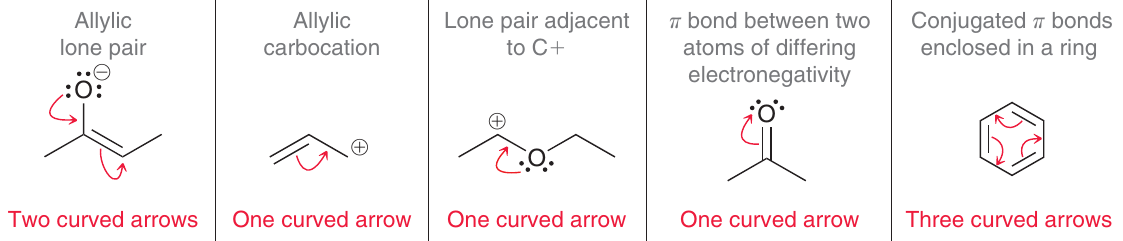
\includegraphics[scale=0.4]{images/patterns.png}
    \end{center}
    \subsubsection{Resonance Hybrid}
    \begin{itemize}
        \item \textbf{Resonance hybrid}: respresents the \textit{average} of the contributing structures, with bond lengths and partial charges taking on intermediate values.
        \item No matter how many resonance structures are drawn, they collectively represent one entity.
        \item Drawn partial bonds and charges to illustrate the delocalization of electrons.
    \end{itemize}
    \subsubsection{Delocalization}
    \begin{itemize}
        \item \textbf{Delocalization}: the spreading of electrons between multiple atoms or covalent bonds.
        \begin{itemize}
            \item \textbf{Resonance stabilization}: molecules and ions that are {\color{o-Sun}stabalized} by the delocalization of electrons.
            \item Plays a major role in the outcome of many reactions.
        \end{itemize}
        \item When a lone pair particpates in resonance, it will occupy a \textit{p} orbtail rather than hybridized; important for 3d shapes of proteins.
        \item \textbf{Localized lone pair}: when a lone pair is not allylic to a $\pi$ bond. 
            \begin{itemize}
                \item Whenever an atom posses both a $\pi$ bond and a lone pair, they will not both participate in resonance.
                \item Usually $\pi$ bonds participate first.
            \end{itemize}
    \end{itemize}
    \subsubsection{Contributor Significance}
    \begin{itemize}
        \item Some resonance structures may resemble the actual molecule more than another, in regards to energy and stability.
        \item Strcures with low potential energy are more stable compared to those of higher values and resemble the actual structure more.
        \item \textbf{Major contributors}: the most stable contributing structures.
        \item \textbf{Minor contributors}: less favorable contributing strcutres.
        \item Rules for contributing significance, descending:
            \begin{itemize}
                \item The greatest number of filled octets.
                \item The greatest number of covalent bonds.
                \item Minimize formally charged atoms.
                \item Separation of unlike and like charges, minimized and maximized respectively.
                \item Negative charges placed on the most electronegativity atoms, positive charges placed on the less electronegative atoms.
                \item Do not deviate substantially from idealized bond lengths and angles.
                \item Maintain aromatic substructures locally while avoiding anti-aromatic ones.
            \end{itemize}
    \end{itemize}
\end{itemize}
%\endgroup
%%%%%%%%%%%%%%%%%%%%%%%%%%%%% Chapter 2 %%%%%%%%%%%%%%%%%%%%%%%%%%%%%

%%%%%%%%%%%%%%%%%%%%%%%%%%%%% Chapter 3 %%%%%%%%%%%%%%%%%%%%%%%%%%%%%
%\begingroup
\clearpage
\section{Acids and Bases}\phantomsection
\subsection{B{\o}nsted-Lowry Acids and Bases}
\begin{itemize}
    \item \textbf{Acid}: a {\color{o-Sun}proton donor}; i.e., a {\color{pos}\ch{H^+}} donor.
    \item \textbf{Base}: a {\color{o-Sun}proton acceptor}; i.e., a {\color{neg}\ch{OH^-}} (hydroxide ion), which wants a {\color{pos}\ch{H^+}} to form the more stable \ch{H2O}.
    \item General definition: {\color{pos}acid} + {\color{neg}base} \ch{<>} {\color{neg}conjugate base} + {\color{pos}conjugate acid}
        \begin{itemize}
            \item Symbolically: {\color{pos}HA} + {\color{neg}B} \ch{<>} {\color{neg}\ch{A^-}} + {\color{pos}\ch{HB^+}}
            \item The strength of the acid/base is {\color{o-Sun}inversley proportional} to the strength of the conjugate acid/base.
        \end{itemize}
    \item Most acid-base reactions are reversible.
        \begin{itemize}
            \item Strong acids tend to be less reversible.
        \end{itemize}
    \item Example using bond-line structures:
        \begin{itemize}
            \item 
            \chemfig{{\color{pos}H}-[:30]O-[:-30]H}
            \hspace{6pt}{\large+}\hspace{6pt}
            \chemfig{-[:30](-[:120])(-[:60])-[:-30]\chemabove{\textcolor{neg}O}{{\color{neg}\scriptstyle\circleddash}}} 
            \hspace{6pt}{\large\ch{<>}}\hspace{6pt}
            {\color{neg}$^\circleddash$O}H
            \hspace{6pt}{\large+}\hspace{6pt}
            \chemfig{-[:30](-[:120])(-[:60])-[:-30]O-[:30]{\color{pos}H}}
    \end{itemize}
    \subsubsection{Quantitative Perspective}
    \begin{itemize}
        \item \textbf{Equilibrium}: when there is no longer an observable change in concentrations of reactants and products.
            \begin{itemize}
                \item \(K_{eq}=\dfrac{[\ch{H3O+}]\,[\ch{A-}]}{[\ch{HA}]\,[\ch{H2O}]}\)
                \item Water concentration is fairly constant and can be removed, giving \(K_a\).
                    \begin{itemize}
                        \item \(K_a=K_{eq}\,[\ch{H2O}]=\dfrac{[\ch{H3O+}]\,[\ch{A-}]}{[\ch{HA}]}\)
                    \end{itemize}
                \item \(K_a\) tends to be large, so it's converted to \(pK_a\).
                    \begin{itemize}
                        \item \(pK_a=-\log{K_a}\)
                        \item Generally ranges from {\color{pos}-10 (strong acid)} to {\color{neg}50 (strong base)}.
                    \end{itemize}
                \item {\color{pos}\(pK_a\) (\ch{H+})} can be easily converted to {\color{neg}\(pK_b\) (\ch{OH-})}:
                    \begin{itemize}
                        \item \(pK_b=14-pK_a\)
                    \end{itemize}
            \end{itemize}
        \item Equilibrium {\color{o-Sun}favors formation} of the {\color{o-Sun} weaker} (higher \(pK_a\)) {\color{o-Sun}acid}.
            \begin{itemize}
                \item Reactions with vastly different \(pK_a\) values make the reverse proccess is negligible.
                \item Can ignore the reverse reaction in such cases and treat it as a reaction in one direction.
            \end{itemize}
    \end{itemize}
    \subsubsection{Qualitiative Perspective}
    \begin{itemize}
        \item Relative acid strength can be determind by comparing conjugate bases. 
            \begin{itemize}
                \item The {\color{o-Sun}more stable} (weaker) the conjugate base, the {\color{o-Sun}stronger} the acid.
                \item Does not predict \(pK_a\), just a means of comparing relative acid strenghts with out known \(pK_a\)
            \end{itemize}
        \item \textbf{Stabilization factors}: (1) {\color{o-Sun}atom bearing the charge}, (2) {\color{o-Sun}resonance}, (3) {\color{o-Sun}induction}, and (4) {\color{o-Sun}orbitals}.
            \begin{itemize}
                \item Generally follow decending order of significance; absence of difference in earlir factors allow for later factors to express more significance.
            \end{itemize}
        \item \textbf{Atom bearing the charge}: Compare atoms bearing negative charge in each conjugate base after deprotonation.
            \begin{itemize}
                \item First determin if atoms are in same row or column in the periodic table.
                \item {\color{o-Sun}Row} comparison: {\color{o-Sun}electronegativity} is the dominant effect; stability is greater when the negative charge is on the {\color{o-Sun}more electronegative} element.
                \item {\color{o-Sun}Column} comparsion: {\color{o-Sun}size} is the dominant effect; stability is greater when the negative charge is on the {\color{o-Sun}larger} element. 
            \end{itemize}
        \item \textbf{Resonance}: charge that is delocalized across multiple atoms will lead to more stable structures comapred to molecules with no resonance.
            \begin{itemize}
                \item Helps determing relative stability when both molecules bare the same elements that have a difference in charge.
                \item Again, more stability means it's the weaker conjugate base, meaning the proton removed from the atom creating the resonance hybrid will be more acidic.
            \end{itemize}
        \item \textbf{Induction}: induction of other atoms can act to withdraw the negative charge away from the new electronegatively charged atom due to deprotonation.
            \begin{itemize}
                \item Inductive effect diminishes the further the electronegative atom is away from the depronated atom.
            \end{itemize}
        \item \textbf{Orbitals}: negative charges on atoms with lower hybridization result in greater stability due to proximity to positive nucleus, i.e., \({\color{neg}sp} > sp^2 > {\color{pos}sp^3}\)
            \begin{itemize}
                \item sp = triple bond, sp\(^{2}\) = double bond, sp\(^{3}\) = three $\sigma$ bonds.
            \end{itemize}
    \end{itemize}
\end{itemize}

\subsection{Lewis Acids and Bases}
\begin{itemize}
    \item The lewis definition is more broad than the Br{\o}nsted-Lowry definition.
    \item Lewis describes acidity in terms of {\color{o-Sun}electrons}, rather than protons.
    \item \textbf{Lewis acid}: electron-pair {\color{o-Sun}acceptor}.
    \item \textbf{Lewis base}: electron-pair {\color{o-Sun}donor}.
    \item All B{\o}nsted-Lowry acids and bases are Lewis acid and bases, but the inverse is not always true.
    \item Most reactions are described in terms of lewis base and acids, since molecules without donatable protons are unable to be described by the Br{\o}nsted-Lowry definition.
\end{itemize}

\subsection{Nucleophiles and Electrophiles}\label{ssec:bar}
{\color{darklc}\textit{Excerpt from Chapter 6: Chemical Reactivity and Mechanisms $\mapsto$}}
\begin{itemize}
    \item \textbf{Ionic reactions}, {\color{G-Moon}aka polar reactions}: reactions that involve the particpation of ions as reactants, intermediates, or products.
        \begin{itemize}
            \item Most cases ions act as intermediates.
            \item Radical reactions and pericyclic reactions are also major categories, but are typically not discussed in undergraduate courses.
            \item Ionic reactions occur when one reactant has a site of {\color{neg}high electron density} and the other reactant has a site of {\color{pos}low electron density}.
        \end{itemize}
    \item \textbf{Nucleophiles}: an electron rich atom that is capable of donating a pair of electrons.
        \begin{itemize}
            \item {\color{neg}Nucleophiles are Lewis bases}.
            \item Any atom that possesses a localized lone pair can be nucleophilic.
            \item $\pi$ bonds can also function as nucleophiles due to their region of space having high electron density.
            \item \textbf{Polarizability}: the ability of an atom to distribute its electron density unevenly in response to external influences.
                \begin{itemize}
                    \item Correlated with size of the atom, which increases the number electrons that are distant from the nucleus.
                \end{itemize}
        \end{itemize}
    \item \textbf{Electrophiles}: an electron-deficient atom that is capable of accepting a pair of electrons.
        \begin{itemize}
            \item {\color{pos}Electrophiles are Lewis acids}.
        \end{itemize}
\end{itemize}

\subsection{Flow of Electron Density: Curved-Arrow Notation}
\begin{itemize}
    \item All reactions are accomplished via a flow of electron density.
    \item Electron density flow is illustrated with curved arrows.
        \begin{itemize}
            \item \textbf{Reaction mechanism}: how the reaction occurs in terms of the motion 
            \item All ionic meachanisms, regardless of complexity, are combinations of four characteristic patterns of electron flow \textit{(discussed later)}.
        \end{itemize}
    \subsubsection{Notes on Drawing Curved Arrows}
    \begin{itemize}
        \item \textbf{Tails} must be placed on either a bond or a lone pair.
            \begin{itemize}
                \item Shows the {\color{o-Sun}source}, i.e., the electron donor (base).
                \item Electrons can only be found in lone pairs or bonds, so {\color{o-Sun}never place the tail} of a curved arrow on a {\color{pos}positive charge}.
            \end{itemize}
        \item \textbf{Heads} must be placed so that it shows either the formation of a bond or the formation of a lone pair.
            \begin{itemize}
                \item Shows the {\color{o-Sun}destination}, i.e., the electron acceptor (acid).
                \item Avoid drawing an arrow that violates the octet rule, so never draw an arrow that gives more than four orbitals to a second-row element.
            \end{itemize}
    \end{itemize}
\end{itemize}

%\endgroup
%%%%%%%%%%%%%%%%%%%%%%%%%%%%% Chapter 3 %%%%%%%%%%%%%%%%%%%%%%%%%%%%%

%%%%%%%%%%%%%%%%%%%%%%%%%%%%% Chapter 4 %%%%%%%%%%%%%%%%%%%%%%%%%%%%%
%\begingroup
\clearpage
\section{Alkanes and Cycloalkanes}\phantomsection
\subsection{Nomenclature of Alkanes}
\begin{itemize}
    \item \textbf{Alkane}: acyclic (linear structure) saturated hydrocarbons (no $\pi$ bonds).
        \begin{itemize}
            \item General chemical formula: {\color{o-Sun}\ch{C_nH_{2n+2}}}
        \end{itemize}
    \item \textbf{Substituents}: branches connected to the parent chain.
    \subsubsection{Selecting the Parent Chain}
    \begin{itemize}
        \item \textbf{Parent chain}: the longest carbon chain in an alkane.
        \begin{table}[h]
            \centering
            \caption{Parent Names for Alkanes\strut}
            \label{tab:alkanes}
            \begin{tabular}{ccc}
                \toprule
                Number of Carbons & Parent & Name \\
                \midrule
                1 & meth & methane \\
                2 & eth & ethane \\
                3 & pro & propane \\
                4 & but & butane \\
                5 & pent & pentane\\
                6 & hex & hexane \\
                7 & hept & heptane \\
                8 & oct & octane \\
                9 & non & nonane \\
                10 & dec & decane \\
                11 & undec & undecane \\
                12 & dodec & dodecane \\
                13 & tridec & tridecane \\
                14 & tetradec & tetradecane \\
                15 & pentadec & pentadecane\\
                20 & eicos & eicosane \\
                30 & triacont & triacontane \\
                40 & tetracont & tetracontane \\
                50 & pentacont & hectane \\
                100 & hect & hectane \\
                \bottomrule
                \end{tabular}
        \end{table}   
    \item \textbf{Substituents}: branches connected to the parent chain, can be a single atom, groups of atoms, that replace one or more hydrogen atoms. 
        \begin{itemize}
            \item If there is competition between chains of {\color{o-Sun}equal length}, then {\color{o-Sun}choose the chain with greatest number of substituents}.
        \end{itemize}
    \item \textbf{Cycloalkanes (cyclo)}: presence of a ring in an alkane.
    \end{itemize}
    \subsubsection{Naming Substituents}
    \begin{itemize}
        \item \textbf{Alkyl groups}: Substituents that are named the same as the parents, but with the added letters {\color{o-Sun}ly}.
        \begin{table}[h]
            \centering
            \caption{Names of Alkyl Groups\strut}
            \label{tab:substituents}
            \begin{tabular}{ccc}
                \toprule
                Substituent Carbons&  Terminology\\
                \midrule
                1 & meth{\color{o-Sun}y}l\\
                2 & eth{\color{o-Sun}yl} \\
                3 & pro{\color{o-Sun}pyl} \\
                4 & but{\color{o-Sun}yl} \\
                5 & pent{\color{o-Sun}yl} \\
                6 & hex{\color{o-Sun}yl} \\
                7 & hept{\color{o-Sun}yl} \\
                8 & oct{\color{o-Sun}yl} \\
                9 & non{\color{o-Sun}yl} \\
                10 & dec{\color{o-Sun}yl} \\
                \bottomrule
                \end{tabular}
        \end{table}
        \item When a group is connected to the ring, then the ring is generally treated as the parent.
            \begin{itemize}
                \item If the ring has fewer atoms the the rest of the structure, then it becomes a substituent.
            \end{itemize}
    \end{itemize}
    \subsubsection{Naming Complex substituents}
    \begin{itemize}
        \item \textbf{Complex substituents}: branched alkyl substituents.
        \item Begin by numbering carbons going {\color{o-Sun}away} from the parent chain, then name it as if its a parent chain itself.
            \begin{itemize}
                \item Complex substituent are placed in parentheses, indicating it as a single substituent of the parent chain.
            \end{itemize}
        \item Some complex substituents have common names that are so well established and allowed by IUPAC.
            \begin{itemize}
                \item An alkyl group bearing {\color{o-Sun}three} carbon atoms; only one way to branch it.
                    \begin{itemize}
                        \item \textbf{Isopropyl group}: (1-methylethyl): {\tiny\chemfig{-[:0](-[::60])-[::-60]}}
                    \end{itemize}
                \item Alkyl groups bearing {\color{o-Sun}four} carbon atoms, which can be branched three different ways:
                    \begin{itemize}
                        \item \textbf{sec-butyl} (1-methylpropyl): {\tiny\chemfig{-[:0](-[::60]-[:0])-[::-60]}}
                        \item \textbf{isobutyl} (2-methylpropyl): {\tiny\chemfig{-[:0](-[::60](-[:120])-[:0])}}
                        \item \textbf{tert-butyl} (1,1-dimethylethyl): {\tiny\chemfig{-[:0](-[::60])(-[:0])(-[::-60])}} 
                    \end{itemize}
                \item Alkyl groups bearing {\color{o-Sun}five} carbons, which can be branched many more ways. Two common ways:
                    \begin{itemize}
                        \item \textbf{isopentyl (isoamyl)} (3-methylbutyl): 
                    {\tiny\chemfig{-[:0]-[::60]-[:0](-[:60])-[:-60]}}
                        \item \textbf{neopentyl} (2,2-dimethylpropyl):
                    {\tiny\chemfig{-[:0]-[::60](-[:-15])(-[:50])(-[:120])}}
                    \end{itemize}
            \end{itemize}
    \end{itemize}
    \subsubsection{Assembling the Systematic Name}
    \begin{itemize}
        \item \textbf{Locant}: the location of a carbon numbered parent chain.
        \item Rules for assinging locant:
            \begin{itemize}
                \item If one substituent is present, then assign the lowest number possbile.
                \item When multiple substituents are present, then the first substituent receives the lowest number. 
                    \begin{itemize}
                        \item If there is a tie, the second locant should be as low as possible.
                        \item If tie cannot be broken, then lowest number is assigned alphabetically.
                    \end{itemize}
                \item Prefixes are used when the same substituent appears more than once. 
                    \begin{itemize}
                        \item di:2, tri:3, tetra:4, penta:5, 6:hexa
                    \end{itemize}
                \item Hypens are used to separate numbers from letters, while commas are used to separate numbers from each other.
                \item Substituents are alphabeticalized after all locants are correctly assigned.
                    \begin{itemize}
                        \item Prefixes are ignored during alphabeticalization.
                    \end{itemize}
            \end{itemize}
        \item Summary of discrete steps:
            \begin{enumerate}
                \item \textbf{Identify parent chain}
                \item \textbf{Identify and name substituents}
                \item \textbf{Number the parent chain and assign a locant to each substituent}
                \item \textbf{Arrange the substituents alphabetically}
            \end{enumerate}
    \end{itemize}
\end{itemize}

\subsection{Constitutional Isomers of Alkanes}
\begin{itemize}
    \item For an alkane, the number of possible constitutional isomers increases with increaseing molecular size.
    \item Determing IUPAC name is the best way to tell if two alkanes are constitutional isomers, or just different representations of the same one.
    \begin{table}[h]
        \centering
        \caption{Constitutional Isomers for Various Alkanes\strut}
        \label{tab:constitutional}
        \begin{tabular}{ccc}
            \toprule
            Molecular Formula &  Constitutional Isomers\\
            \midrule
            \ch{C3H8} & 1\\
            \ch{C4H10} & 2\\
            \ch{C5H12} & 3\\
            \ch{C6H14} & 5\\
            \ch{C7H16} & 9\\
            \ch{C8H18} & 18\\
            \ch{C9H20} & 35\\
            \ch{C10H22} & 75\\
            \ch{C15H32} & 4,347\\
            \ch{C20H42} & 366,319\\
            \ch{C40H62} & 4,111,846,763\\
            \bottomrule
            \end{tabular}
    \end{table}
\end{itemize}

\subsection{Newman Projections}
\begin{itemize}
    \item \textbf{Conformations}: the variety of possible three-dimensional shapes of a molecule that are interchangeable by low energy pathways.
        \begin{itemize}
            \item Conformations vary in potential energy.
            \item Changes due to rotation about $\sigma$ bonds.
        \end{itemize}
    \item \textbf{Configurations}: refer to different orientations in space that require breaking of bonds (high energy pathway) to change.
        \begin{itemize}
            \item Cis and trans isomers in alkenes (\textit{discussed later})
        \end{itemize}
    \item \textbf{Newman projections}: a type of representation of compounds specially designed for showing the conformation of a molecule.
        \begin{itemize}
            \item Drawn from the angle of the observer, with the front carbon represented in front of the circle, and the back carbon behind the circle.
            \item ***Chemmacros package is broken due to font usage, need to figure out how to fix that before inserting drawings***
        \end{itemize}
    \subsubsection{Conformational Analysis of Ethane and Propane}
    \begin{itemize}
        \item \textbf{dihedral (torsional) angle}: the angle between substituents of front and back carbons as the $\sigma$ bonds rotates.
        \item There are an infinite number of possbile conformations, but there are conformations of maximum and minium energy.
            \begin{itemize}
                \item \textbf{Staggered conformation}: {\color{o-Sun}lowest energy} conformation, when two substituents are at maximum dihedral angle from each other.
                \item \textbf{Eclipsed conformation}: the {\color{o-Sun}highest energy} conformation, when two substituents are at the minimum dihedral angle from each other.
            \end{itemize}
        \item \textbf{Degenerate}: when all staggered conformations have the same amount of energy.
            \begin{itemize}
                \item All staggered and eclipsed conformations of ethanes are degenerate.
            \end{itemize}
        \item \textbf{Torsional strain}: the difference in energy between staggered and eclipsed conformations.
            \begin{itemize}
                \item Recent quantum methods suggest conformation possesses a favorable interaction between occupied, bonding molecular orbitals and unoccupied, antibonding molecular orbitals.
                \item An increase in potential energy occurs when the favorable overalp is broken.
                \item A sample of ethane gas at room temperature will have \(\approx\) 99\% of its molecules staggered.
            \end{itemize}
        \item Ethane has total cost of \SI{12}{kJ\per\mole} (\SI{4}{kJ\per\mole\per H}), while propane has total cost of \SI{14}{kJ\per\mole}.
            \begin{itemize}
                \item Reasonable estimates of energy cost of an H eclipsing a \ch{CH3} group must be \SI{6}{kJ\per\mole}.
            \end{itemize}
    \end{itemize}
    \subsubsection{Conformational Analysis of Butane}
    \begin{itemize}
        \item Butane has three eclipsed conformations that are {\color{o-Sun}not degenerate}.
            \begin{itemize}
                \item Dihedral angle of \ang{0} has the highest eclipsed energy, while both conformations at \(\pm\)\ang{120} are second highest in energy and degenerate.
                \item Likewise, a dihedral angle of \ang{180} has the lowest staggered energy, while both conformations at \(\pm\)\ang{60} are second lowest in energy and degenerate.
            \end{itemize}
        \item \textbf{Anti conformation}: the conformation with a dihedral angle of \(180\); the lowest staggered energy.
            \begin{itemize}
                \item Occurs when the methyl groups are farthest apart.
            \end{itemize}
        \item \textbf{Steric interaction}: nonbonding intereactions that influences energy levels conformations.
        \item \textbf{Gauche interaction}: unfavorable intereaction between substituents, causing an increases in energy due to electron cloud repulsion.
            \begin{itemize}
                \item Gauche intereaction is a type of steric intereactions present at \(\pm\ang{60}\) of the next eclipsed conformation.
            \end{itemize}
        \item Costs of butane: \SI{19}{kJ\per\mole}, \SI{16}{kJ\per\mole}, \SI{3.8}{kJ\per\mole}
            \begin{itemize}
                \item Energy cost of eclipsing \ch{CH3}/\ch{CH3}: \SI{11}{kJ\per\mole}
                \item Energy cost for gauche interaction of \ch{CH3}/\ch{CH3} \SI{3.8}{kJ\per\mole} for butane.
                \item Energy cost of eclipsing \ch{CH3}/H: \SI{6}{kJ\per\mole} 
                \item Energy cost of eclipsing H/H: \SI{4}{kJ\per\mole} 
            \end{itemize}
    \end{itemize}
\end{itemize}

\subsection{Cycloalkanes}
\begin{itemize}
    \item \textbf{Angle strain}: the increases in energy associated with a bond angle that has deviated from the preferred angle of \ang{109.5}. 
        \begin{itemize}
            \item Cyclic alkanes, excpet cyclopropane, are {\color{o-Sun}not planar}. 
            \item Expected angels are different than origanally proposed by Adolph von Baeyer, which assumed rings were planar.
            \item Angle strain is only one factor that contributes to the energy of various ring sizes.
        \end{itemize}
    \item \textbf{Cyclopropane}:
        \begin{itemize}
            \item Under significant angle strain.
            \item Locked into an eclipsed conformation due to triangular structure; exhibiting significant torsional strain.
            \item Thus highly reactive and very susceptible to ring-opening reactions.
        \end{itemize}
    \item \textbf{Cyclopentane}: 
        \begin{itemize}
            \item Less angle strain than cyclopropane. 
            \item More torsional strian than cyclopropane due to four sets eclipsing hydrogens.
            \item Adopts slightly "puckered" shape, which is the cause of reduced angle strain.
        \end{itemize}
    \item \textbf{Cyclopentane}:
        \begin{itemize}
            \item Less total strain than both cyclopropane and cyclopentane.
            \item Can adopt a relatively low strained conformation.
        \end{itemize}
    \subsubsection{Conformations of Cyclohexane}
    \begin{itemize}
        \item \textbf{Chair conformation}:
            \begin{itemize}
                \item Bond angles close to \ang{109.5}; little angle strain.
                \item No torsional strain; all hydrogens are staggered.
                \item Least potential energy of cyclohexane conformations.
                \item \textbf{Half-chair}: highest potential energy, formed via interchange between alternate chair form; leads into twisted boat.
            \end{itemize}
        \item \textbf{Boat conformation}: 
            \begin{itemize}
                \item Bond angles also close to \ang{109.5}; little angle strain.
                \item Two sources of torsional strain; many of hydrogens are eclipsed.
                \item One hydrogen on each side experiences a steric interaction called the {\color{o-Sun}flagpole intereaction}.
                \item Second highest potential energy.
                \item \textbf{Twisted boat}: second lowest potential energy, a slightly less strained version of boat that avoids some of the flagpole interaction.
            \end{itemize}
        \item Majority of cyclohexanes are found in chair form. All other forms are intermediates between alternate chair forms.
    \end{itemize}
    \subsubsection{Drawing Chair Conformations}
    \begin{itemize}
        \item \chemfig{?-[:-50]-[:10]-[:-10]-[:130]-[:190]?}
        \item \textbf{Axial position}: parallel to a vertical axis passing through the center of the ring.
            \begin{itemize}
                \item less stable than equatorial due to steric strain.
            \end{itemize}
        \item \textbf{Equatorial}: positioned approximately along the equator of the ring.
                \item \chemfig{?
                (-[:90,0.7,,,r-Sun, line width=1pt])
                (-[:190,0.7,,,neg, line width=1pt])
                -[:-50](-[:-90,0.7,,,r-Sun, line width=1pt])
                (-[:170,0.7,,,neg, line width=1pt])
                -[:10](-[:90,0.7,,,r-Sun, line width=1pt])
                (-[:300,0.7,,,neg, line width=1pt])
                -[:-10](-[:-90,0.7,,,r-Sun, line width=1pt])
                (-[:10,0.7,,,neg, line width=1pt])
                -[:130](-[:90,0.7,,,r-Sun, line width=1pt])
                (-[:-10,0.7,,,neg, line width=1pt])
                -[:190]
                ?(-[:-90,0.7,,,r-Sun, line width=1pt])
                (-[:120,0.7,,,neg, line width=1pt])}
        \item The chair is more stable when the methyl (substituent) group is in the {\color{o-Sun}equatorial} position.
            \begin{itemize}
                \item The larger the substituent, the more equatorial-substituted conformer is favored.
            \end{itemize}
    \end{itemize}
\end{itemize}
%\endgroup
%%%%%%%%%%%%%%%%%%%%%%%%%%%%% Chapter 4 %%%%%%%%%%%%%%%%%%%%%%%%%%%%%
%\endgroup
\end{document}